\documentclass[a4paper]{article}

\usepackage{graphicx}
\graphicspath{{/}}

\usepackage{subfiles}

\title{Konzeption eines intelligenten, automatischen Fahrradparksystems}
\author{Paul Hartmann, Joshua Lung, Lukas Madlener}
\date{2022/23}


\begin{document}
\maketitle

\break

\subfile{includefile.tex}

\section{Eidesstaatliche Erklärung}
lorem ipsum dolor sit amet


\begin{figure}[h]
  \centering
  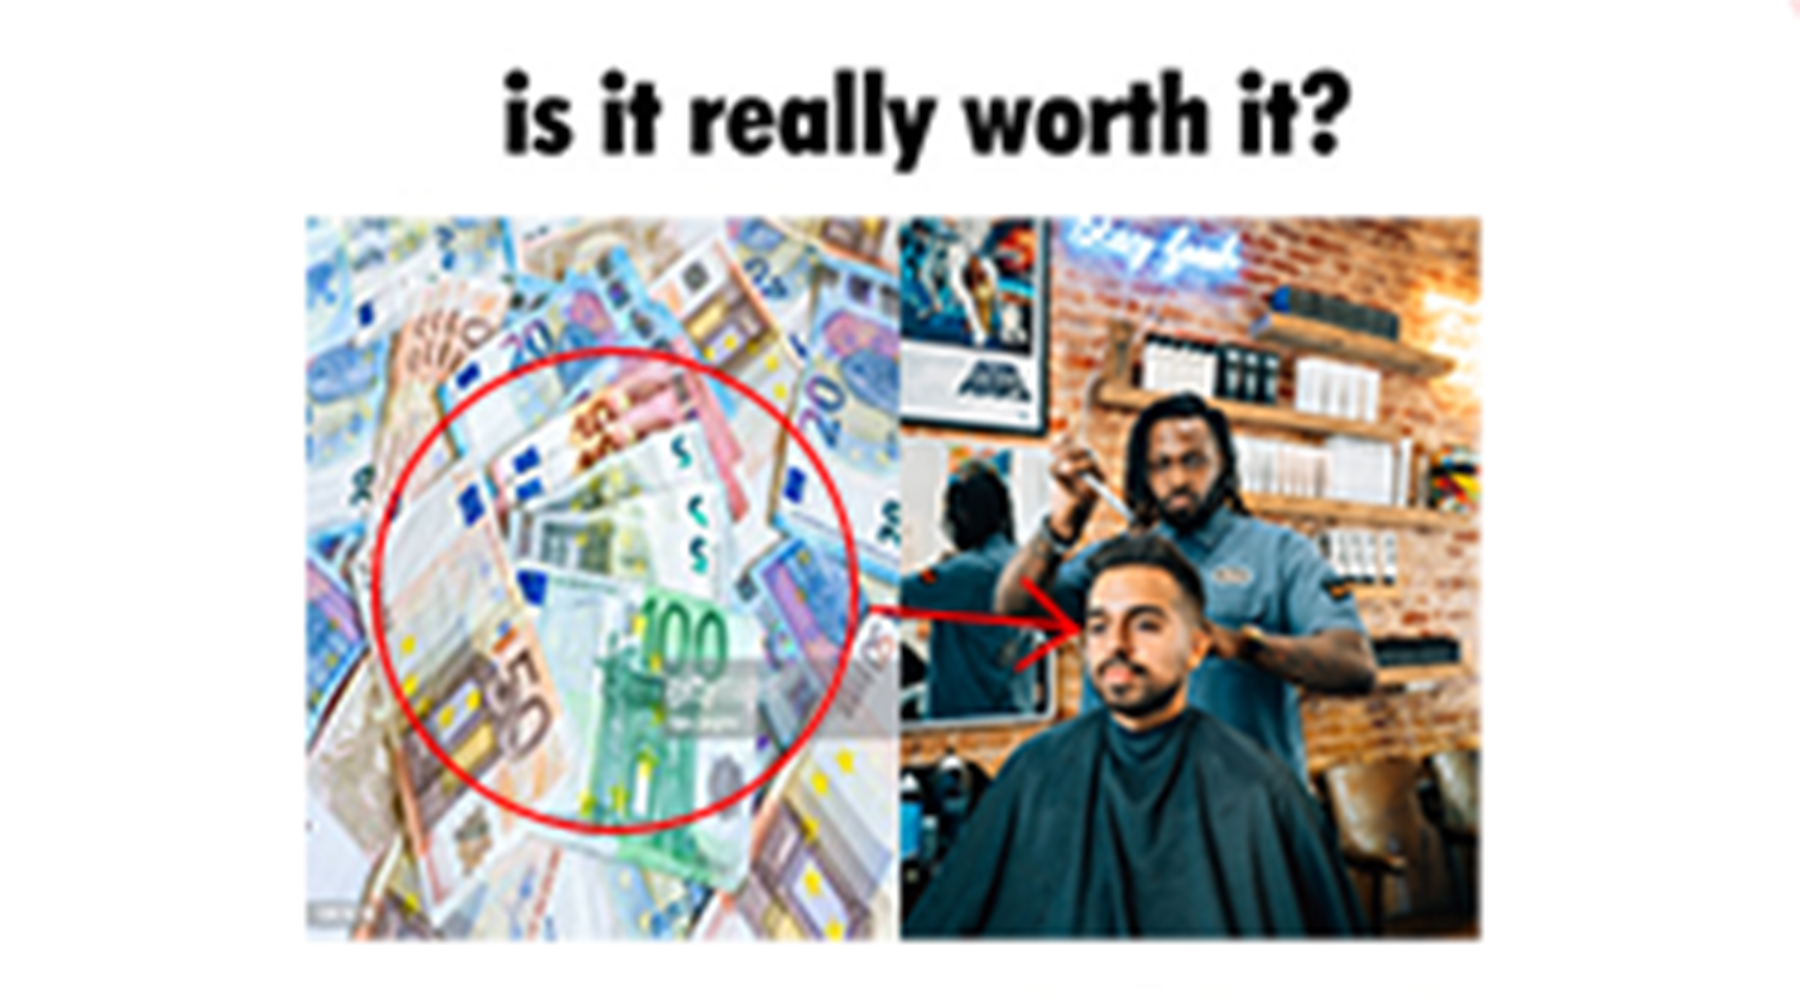
\includegraphics[width=0.75\textwidth]{images/test}
  \caption{Is it worth it?}
  \label{fig:barber_cost}
\end{figure}

As you can see in figure \ref{fig:barber_cost}, the function grows near the origin. This example is on page \pageref{fig:barber_cost}.

\begin{itemize}
  \item crazy item
  \item amogus
  \item more bullets
\end{itemize}

\begin{enumerate}
  \item crazy item
  \item amogus
  \item more bullets
\end{enumerate}

this is a crazy math equation: $x^2 + y^2 = z^2$, it can be inline.

\begin{math}
  x^2 + y^2 = z^2
\end{math}


\begin{abstract}
  This is a simple paragraph at the beginning of the 
  document. A brief introduction about the main subject.
  \end{abstract}

\section{Vorwort}

\section{Inhaltsverzeichnis}
\tableofcontents

\section{Danksagung}

\section{Einleitung}

\section{Hauptteil}

\subsection{Problemstellung}

\subsection{Theoretischer Teil}

\subsubsection{Existierende Modelle}

\subsubsection{Konzept}

\subsection{AAA}

\section{Zusammenfassung}

\section{Literatur- und Quellenverzeichnis}

\section{Abbildungsverzeichnis}

\section{Tabellenverzeichnis}

\section{Abkürzungsverzeichnis}

\section{Begleitprotokoll}

\section{Anhang}

\end{document}